% DMCP Studio -- AAAI 2027 Demonstrations track.
% Two-page short paper + one page of references, AAAI two-column style.
% Single self-contained .tex (AAAI requires no \input for the final source).
% Build: pdflatex main && bibtex main && pdflatex main && pdflatex main
%
% Named build (single-blind demo track). For an anonymous review copy, add the
% [submission] option to the aaai2027 package below (it blanks the byline and
% suppresses the copyright slug); note the hosted-demo URL de-anonymizes anyway.

\documentclass[letterpaper]{article} % DO NOT CHANGE THIS
\usepackage{aaai2027}  % DO NOT CHANGE THIS
\usepackage[hyphens]{url}  % DO NOT CHANGE THIS
\usepackage{graphicx} % DO NOT CHANGE THIS
\urlstyle{rm} % DO NOT CHANGE THIS
\def\UrlFont{\rm}  % DO NOT CHANGE THIS
\usepackage{natbib}  % DO NOT CHANGE THIS
\usepackage{caption} % DO NOT CHANGE THIS
\frenchspacing  % DO NOT CHANGE THIS
\usepackage{amssymb} % for \rightleftharpoons in text

\pdfinfo{
/TemplateVersion (2027.1)
}

\setcounter{secnumdepth}{0}

\title{DMCP Studio: An Interactive, Trace-Grounded Studio for\\
  Effect-Scored Evaluation of LLM Agents over Live MCP Servers}

\author{
    Artem Kuznetsov\equalcontrib\textsuperscript{\rm 1},
    Ilya Galyukshev\equalcontrib\textsuperscript{\rm 1,\rm 2},
    Jerzy Kami\'nski\corresponding\textsuperscript{\rm 1},
    Sergey Chuprin\textsuperscript{\rm 1},\\
    Kirill Redko\textsuperscript{\rm 1},
    Aidar Shumbalov\textsuperscript{\rm 1},
    Anna Kalyuzhnaya\textsuperscript{\rm 1}
}
\affiliations{
    \textsuperscript{\rm 1}ITMO University\quad
    \textsuperscript{\rm 2}Central University\\
    jkaminski@niuitmo.ru
}

\begin{document}
\maketitle

\begin{abstract}
Benchmarks for LLM agents over Model Context Protocol (MCP) servers usually
grade the final answer against a reference string or check a fixed list of
expected tools. Both break once the servers are live and stateful: an answer
goes stale when it depends on today's data, and a fixed tool list penalizes an
agent for a different but equally valid route. DMCP Studio
is an interactive system that makes an alternative visible and inspectable ---
grade the effects an agent produces, not its answer. A visitor drives the full
pipeline (collect, explore, distill, score), then toggles between effect-based
and answer-based grading of one recorded run and watches the verdict flip. A
LIVE/REPLAY switch backs every stage with either the real pipeline or
deterministic fixtures, so the demo is reproducible on a booth laptop yet
provably live.
\end{abstract}

\begin{links}
  \link{Demo}{https://huggingface.co/spaces/jrzkaminski/dmcp-studio}
  \link{Code}{https://github.com/ITMO-NSS-team/DynamicMCPBench}
  \link{Extended version}{https://arxiv.org/abs/2607.20531}
  \link{Video}{https://www.youtube.com/watch?v=66AI1SUrCA8}
\end{links}

\section{Introduction}

Agent systems are increasingly built over MCP servers --- file stores,
databases, and web services behind a uniform calling interface. The practical
question is not whether an agent can issue one tool call, but whether the
configured agent--server stack accomplishes a goal across several interacting
services. Yet most MCP benchmarks score one of two proxies: the agent's final
natural-language answer against a reference string, or the set of tools it was
expected to call \citep{fan2025mcptoolbench++, mo2025livemcpbench, wang2025mcp,
bandi2026mcp}. Both are fragile where deployment matters. A reference answer
goes stale the moment it depends on live data --- today's price, this morning's
commit, the current contents of a table --- and a fixed tool list cannot be
recovered from the prompt alone, so it accumulates spurious ``required'' tools
that penalize a correct agent for a different route. Reproducible tool
environments fight drift by freezing responses \citep{guo2024stabletoolbench,
lu2025toolsandbox, yao2024tau} and generators build corpora from tool
graphs \citep{liu2025mcpeval, shen2024taskbench}, but each still grades an
answer, an outcome, or a tool selection.

The companion methodology \citep{dynamicmcpbench2026} argues that the organizing
object should be neither the answer nor the tool list but the execution trace:
explore a goal live, distill the successful trajectory into path-agnostic
\emph{effect checkpoints}, and grade a candidate only on whether it reproduces
those effects. What a reader does not see from tables is the moment a fluent,
confident answer is marked \textsf{FAILED} because a required effect never
occurred, or a wrong answer marked \textsf{SOLVED} because the live data moved.

DMCP Studio makes that pipeline interactive and its verdicts inspectable. The
methodology --- trace-grounded, effect-scored evaluation --- is the contribution
of the companion paper; the contribution here is the system built on it:
(i)~a browser studio that exposes the full pipeline end to end; (ii)~an
Effect\,$\rightleftharpoons$\,Answer toggle that re-grades one recorded run both
ways and flips the verdict on screen; (iii)~Benchmark Advisor, a pre-generation
statistical planner; and (iv)~a LIVE/REPLAY design that is booth-reproducible
yet demonstrably live. What is new is the system and its evaluation, not the
scoring method.

\section{Effect-Based Scoring}

A \emph{checkpoint} is not a required reference call; it is an observable effect
the reference run produced, together with its admissible realizations. Two kinds
occur. A \emph{tool effect} is met when some tool from an \emph{equivalence set}
runs with arguments that satisfy stated constraints --- for example, the
one-year price-history effect is met by either \texttt{download} or
\texttt{get\_price\_history}. A \emph{value-produced effect} is met when a
required piece of evidence the spec demands appears in the run, matched against
that demand rather than against a gold answer string.

\paragraph{Distillation.} A distiller compiles a recorded successful trace into
a TaskSpec by driving an LLM through a tool-call schema at temperature~0. Because
every checkpoint is derived from a tool that was actually used to reach the goal
--- generation is forward, not sampled from a dependency graph --- a spurious
``unnecessary tool'' cannot appear. The same pass groups tools that produce the
same effect into equivalence sets, records argument constraints, adds
forbidden-action minefields, and infers a partial order over checkpoints.

\paragraph{Matching.} A candidate is run with tool names stripped from its
prompt, and its own trace is scored against the checkpoint ledger by
deterministic field-matching (Tier-1): a checkpoint is met when an admissible
realization appears with satisfying arguments and in an order consistent with
the partial order; triggering a minefield fails the run. Tier-1 uses no model
and no network, so it is exactly reproducible. An optional Tier-2 layer relaxes
strictness --- deterministic \texttt{difflib} comparison for near-miss values
plus an LLM effect-equivalence judge --- and is kept off the demo's headline
path; the verdict on screen is Tier-1.

\section{The Studio}

\begin{figure}[t]
\centering
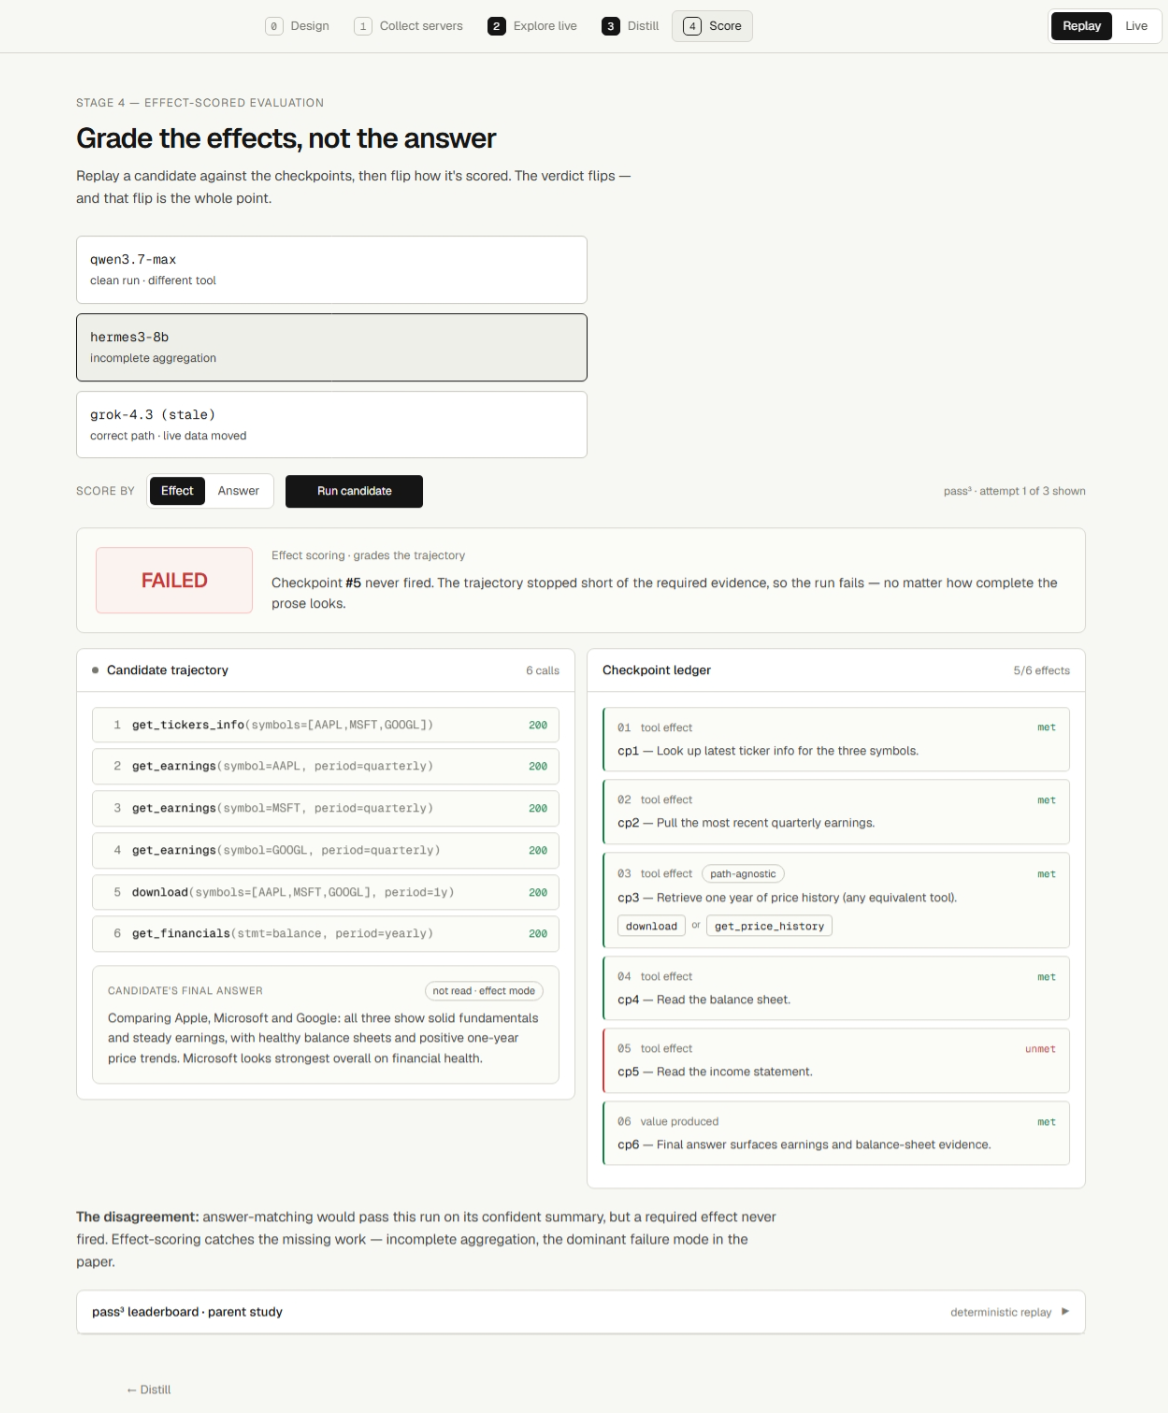
\includegraphics[width=0.63\columnwidth]{figures/fig_studio.png}
\caption{Scoring stage in REPLAY. The \textsf{hermes3-8b} candidate is marked
  \textsf{FAILED}: its trajectory (left) reaches every effect except the
  income-statement checkpoint (\#5, unmet in the ledger, right), though its prose
  summary would pass answer-matching. The Effect\,$\rightleftharpoons$\,Answer
  toggle re-grades the same recorded run without a second backend call.}
\label{fig:studio}
\end{figure}

A single-page front end talks to a FastAPI back end that wraps the
published pipeline through thin adapters, never reimplementing distillation or
scoring; the two slow stages stream call-by-call over Server-Sent Events, so the
interface fills as the agent acts. Four stages follow one another
(Figure~\ref{fig:studio}). \emph{Collect}
points the studio at MCP servers and tags each tool by dynamism (live-read
vs.\ stateful-write). \emph{Explore} turns the tool surface into a realistic
goal and pursues it live, streaming a reference trace. \emph{Distill} compiles
that trace into a TaskSpec, rendering each checkpoint as a card and each
equivalence set as an editable chip. \emph{Score} replays a candidate against
the ledger; the endpoint returns both an effect verdict and an answer-matching
baseline on every call, so the Effect/Answer toggle is a pure front-end
re-render rather than a second backend call, and toggling an equivalence-set
member re-scores live.

\paragraph{Stage 0: Benchmark Advisor.} Planning a corpus with adequate power is
the first step of building a defensible effect benchmark, so before generation
the Advisor turns an evaluation question into a scoped statistical plan. Its core
diagnostic is the pre-run minimum detectable effect, computed over the number of
\emph{unique} tasks: repeated attempts support reliability analysis but do not
multiply the independent sample size, so a 40-task smoke run and a 500-task
selection run make visibly different claims before either is launched.
Under-powered or unsafe plans are refused or repaired, and only approved plans
carry into generation.

\paragraph{The verdict flip.} The studio is organized around making the two
scoring rules disagree on screen. Three frozen fixtures each reproduce a
different disagreement: an \emph{equivalent-tool pass}, where the candidate
reaches the price-history effect through the other member of the equivalence set;
an \emph{answer-pass / effect-fail}, where a fluent agent skips a required step
yet writes a confident summary (incomplete aggregation, the dominant failure
mode in the parent study); and an \emph{answer-fail / effect-pass}, where a
correct agent reports live returns that no longer match the stored reference.

\paragraph{LIVE vs.\ REPLAY.} A header switch backs every stage with real
pipeline calls or frozen fixtures. In REPLAY --- the public default --- the
deterministic stages, distill and score, recompute over frozen inputs by running
the real pipeline code, so the verdict shown is computed rather than stored;
the slower or non-deterministic stages (collection, goal generation, and the
live exploration stream) are served from recorded fixtures. LIVE drives the whole
pipeline against read-only servers as proof, falling back per stage to the
REPLAY fixture on timeout. A default-deny rule blocks any tool on a
state-changing (\texttt{stateful\_write}) server unless it is flagged sandboxed,
so no real state is modified; the system handles no personal data and is
Apache-2.0 licensed.

\section{Validity and Performance}

The studio's job is to expose the methodology faithfully, and two checks support
that. First, fidelity: across 118 deterministic \emph{(task, candidate)} pairs
the studio reproduces the batch pipeline's Tier-1 verdict exactly --- overall and
on all 708 per-checkpoint comparisons --- so the interface shows the pipeline's
own scorer, not a re-implementation. Second, the effect scorer itself is
validated in the companion study \citep{dynamicmcpbench2026}: annotators reviewed
all 750 results of the strongest locally served model (975 cards). Of the
automatic passes, 94.9\% are confirmed by a human, and the disagreement is
one-sided --- a wrong run is almost never scored as a pass --- with Gwet's AC1
grader agreement of 0.76. Because the reference answer is fully correct only
about 79\% of the time, grading the final answer would wrongly penalize roughly
one task in five: the failure the verdict flip makes visible. Every REPLAY stage
runs in sub-millisecond compute, well within interactive latency; first-time
users reached the verdict flip unaided in an informal walkthrough, and a
structured study is left to future work.

\bibliography{custom}

\end{document}
